\documentclass{beamer}
\usepackage[utf8x]{inputenc}
\usepackage{default}
\usepackage{verbatim}
\newcommand{\Ardrone}{Ar Drone$^{\copyright}$ }

\title{Autonomous Flight With the \Ardrone drone}
\author{Maarten Inja and Maarten de Waard}
\institute{UvA}
\usetheme{Warsaw}
\newcommand{\slide}[2]
{
\begin{frame}
\begin{block}{#1} 

#2

\end{block} \end{frame}
}



\begin{document}
\begin{frame}
\titlepage
\end{frame}

\section{Introduction}


% wat is de ardrone?
% wat willen we er mee doen?
% hoe gaan we dat doen?
% 
% wat is allemaal gelukt?


\slide{The \Ardrone}{
The \Ardrone is an over WiFi remote controlled quadrocopter that has several onboard sensors:
\begin{itemize}
	\item One vertical camera, pointing downwards
	\item One horizontal camera, pointing forward 
	\item Ultrasound altimeter, to measure the altitude
    \item 3 axis accelerometer (measures propellor acceleration)
    \item 2 axis gyrometer 
    \item 1 yaw precision gyrometer
\end{itemize}
Furthermore, it has an onboard computer system running Linux. 

% PROP HIER PLAATJES VAN DE AR DRONE

}

\slide{Our Goal}{
Summer-IMAV 2011 Indoor competition, some sub-tasks of the exploration challenge:
\begin{itemize}
    \item Pick-up Object
    \item Exit Building
    \item Release Object
\end{itemize}

% PROP HIER DAT PLAATJE BIJ VAN DE SETTING

}

\slide{Controlling The Drone}{
\begin{itemize}
    \item Direct Control
        \begin{itemize}
            \item Sending AT-Commands to ports
            \item Listening on different ports to decode navigation data and video
        \end{itemize}
    \item SDK, the Software Development Kid
        \begin{itemize}
            \item A complete framework that takes care of decoding and encoding
            \item Over complicated
            \item Othermans work
        \end{itemize}
    \item Extending C with Python
        \begin{itemize}
            \item We are better at Python
            \item Python seems like a better choice
        \end{itemize}
\end{itemize}
}

\slide{Finding The Object}{
To find the object the drone complete a search pattern
\begin{itemize}
    \item Go to altitude X
    \item Rotate 360 degrees
    \item If the object has not been found, increase altitude X and repeat
\end{itemize}
}

\slide{Recognizing The Object}{
\begin{itemize}
    \item Convert video frame to HSV
    \item Discard pixels that do not match the color of the object
    \item Template match to find the middle of the object
    \item Calculate the distance by calculating the amount of pixels
\end{itemize}
}

\slide{Pick Up The Object}{
\begin{itemize}
    \item Centre the object in the middle of the screen
    \item Fly towards the object
    \item Hover in front of the object at a distance of 0.5 metre for some time to stabilize
    \item Fly above the object to pick it up
\end{itemize}
}



\begin{comment}
\begin{frame}
\frametitle{Measures}

The only thing i need to show you:

  \begin{picture}(0.0,0.0) 
     \put(0.0,-100.0){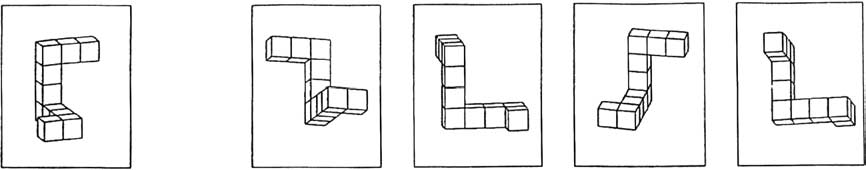
\includegraphics[width=1\textwidth]{mrtitem.png}}
  \end{picture}
\end{frame}


\begin{frame}
  \begin{picture}(0.0,0.0) 
     \put(0.0,100.0){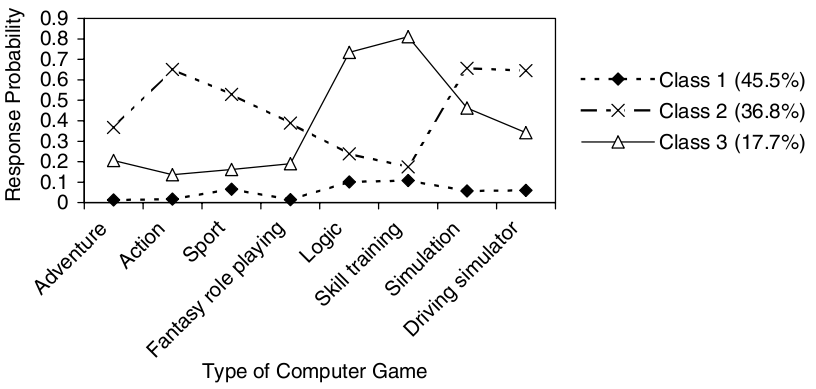
\includegraphics[width=1\textwidth]{fig1.png}}
  \end{picture}
\end{frame}
\end{comment}



\end{document}
